\documentclass{article}
\usepackage[utf8]{inputenc}
\usepackage{geometry}
 \geometry{%
    a4paper,%
    left=25mm,right=25mm,%
    top=25mm,bottom=25mm,%
 }
\usepackage{amsmath}
\usepackage{amssymb}
\usepackage{amsfonts}
\usepackage{hyperref}
 \hypersetup{%
    colorlinks,%
    citecolor=black,%
    filecolor=black,%
    linkcolor=black,%
    urlcolor=blue
 }
\usepackage{tikz}
  \usetikzlibrary{shapes, calc, intersections, spy, external}
  \tikzexternalize[prefix=img/extern/]  % requieres -shell-escape 
\usepackage{pgfplots}
  \pgfplotsset{compat=1.16}
\usepackage{circuitikz}
\usepackage{tikz-timing}
\usepackage{siunitx}
\usepackage{minted}
 \setminted{linenos, breaklines}
\usepackage{caption}

\tikzset{new spy style/.style={spy scope={%
 magnification=5,
 size=1.25cm, 
 connect spies,
 every spy on node/.style={rectangle,draw},
 every spy in node/.style={draw,rectangle,fill=gray!40}
}}}

\newcommand*{\subb}[1]{\ensuremath{_{\mathrm{#1}}}}
\newcommand*{\supp}[1]{\ensuremath{^{\mathrm{#1}}}}
\renewcommand*{\j}{\ensuremath{{\mathrm{j}}}}
\renewcommand\listingscaption{Sample Code}

\title{IL2239 Course Project}
\author{Jordi Altayó \\\texttt{jordiag@kth.se}\and Björn Sunedahl\\\texttt{sunedahl@kth.se}}
\date{January 2019}

% please, use 1 space as indentation
\begin{document}
 \maketitle
 \section*{Introduction}
 The goal of this project is to design a SAR-ADC (Successive Approximation Register Analog to Digital Converter) that meets the following specifications:
 \begin{itemize}
  \item Comparator clock: 100 MHz
  \item $\mathrm{SNDR} > 28$ dB, $\mathrm{SFDR} > 37$ dB
  \item Technology: 150 nm CMOS
  \item Supply voltage: 1.8 V
  \item Input amplitude $V\subb{in}=\SI{0.5}{\volt_{pp}}$
  \item A common-mode input voltage in the range $0 \le V\subb{in,cm} \le 1.8$ V
  \item Voltage reference value: $V\subb{ref}<1.8$ V
  \item Switching energy for a full conversion cycle: \textless 30 pJ for $V\subb{in}=300$ mV (DC)
  \item Resolution: 5 bits
 \end{itemize}
 The circuit topology for the SAR-ADC is given in \autoref{fig:sar}.\bigskip

 \noindent The project will be carried out in several steps (milestones).

 \begin{figure}[!h]
  \centering
  \tikzsetnextfilename{sar}
  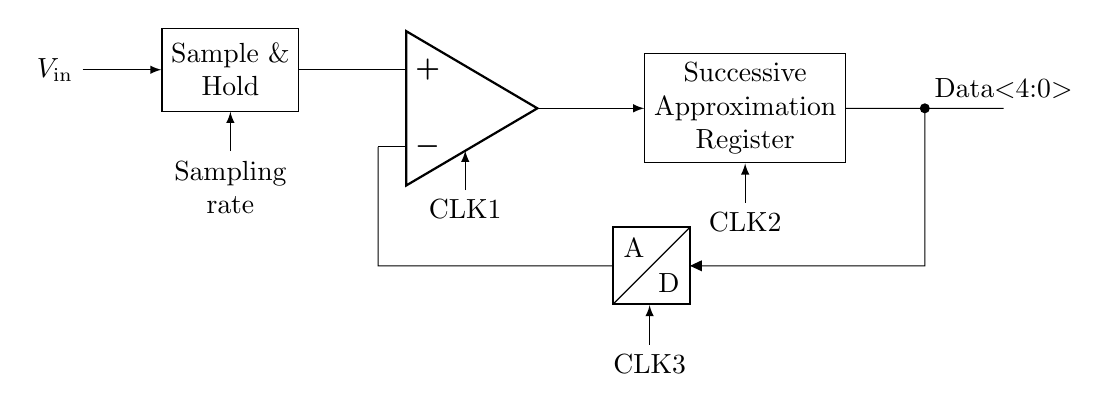
\begin{tikzpicture}
 \draw[-latex] (0,0) node[left] {$V\subb{in}$} --++ (1,0) node[draw, rectangle, minimum height=3em, anchor=west, align=center] (sh) {Sample \&\\Hold};
 \draw (sh.east) --++ (1,0) node[op amp, noinv input up, anchor=+] (opamp) {};
 \draw[-latex] (opamp.out) --++ (1,0) node[draw, rectangle, minimum height=3em, anchor=west, align=center] (sar) {Successive\\Approximation\\Register};
 \draw (sar.east) --++ (1,0) --++ (0,-2) coordinate (a) to[dac,>] (a-|opamp.-) -- (opamp.-);
 \draw (sar.east) ++ (1,0) to[short,*-] ++ (1,0) node[above] {Data\textless 4:0\textgreater};
 \draw[-latex] (sh.south) ++ (0,-0.5) node[below, align=center] {Sampling\\rate} -- (sh.south);
 \draw[-latex] (opamp.down) ++ (0,-0.5) node[below] {CLK1} -- (opamp.down);
 \draw[-latex] (sar.south) ++ (0,-0.5) node[below] {CLK2} -- (sar.south);
 \draw[-latex] (7.2,-2.99) ++ (0,-0.5) node[below] {CLK3} --++ (0,0.5);
\end{tikzpicture} 

  \caption{Block diagram of the SAR-ADC}
  \label{fig:sar}
 \end{figure}

 \section*{Milestone 1}
 \setcounter{section}{1}
 For this milestone the goals are:
 \begin{itemize}
  \item Design a comparator for the given clock frequency.
  \item Choose a common-mode input voltage for the comparator, taking into account the properties of the sample \& hold circuit.
 \end{itemize}
 The comparator used will be of the StrongARM latch topology. To assist us with the design, template projects in Cadence Virtuoso were provided to us.\bigskip

 \noindent The schematic for the StrongARM latch comparator is given in \autoref{fig:sar_schematic}.
 In addition to the comparator schematic, two different testbenches (shown in Figures \ref{fig:tb1}-\ref{fig:tb2}) were provided.

 \begin{figure}[!h]
  \centering
  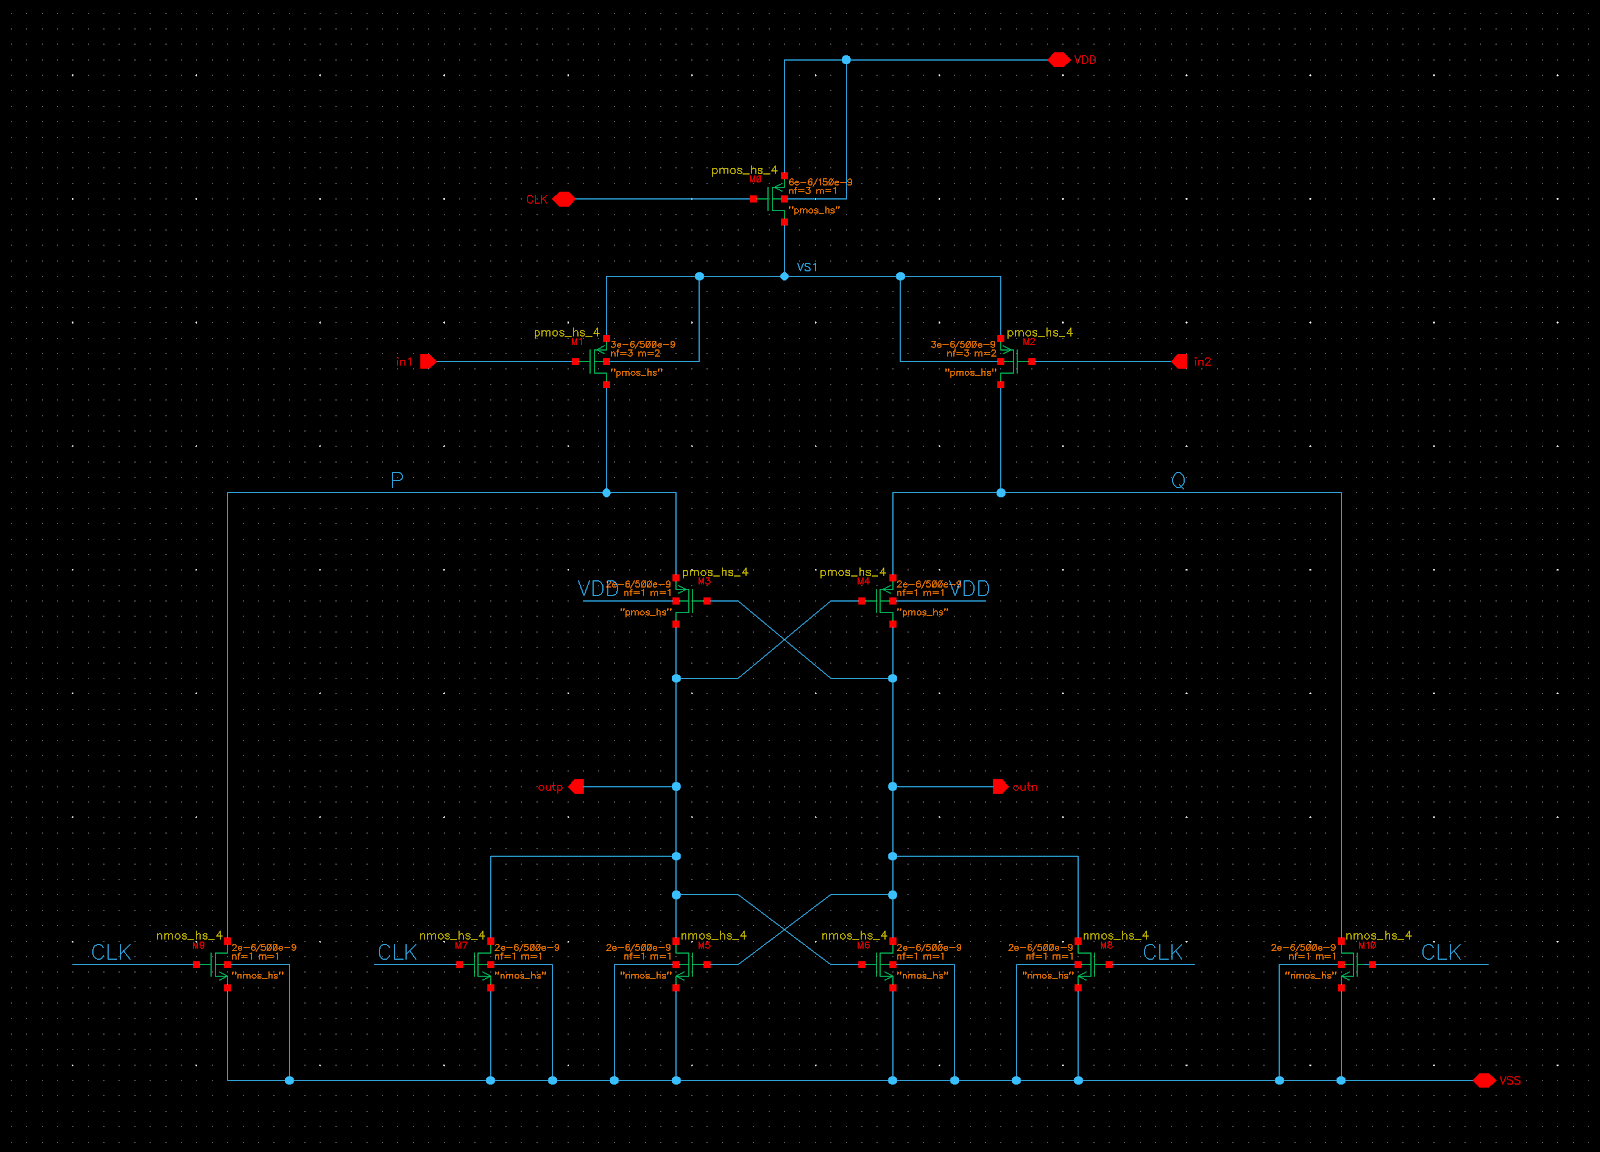
\includegraphics[width=0.8\textwidth]{img/sch}
  \caption{Schematic of the SAR comparator}
  \label{fig:sar_schematic}
 \end{figure}
 
 \begin{figure}[!h]
  \centering
  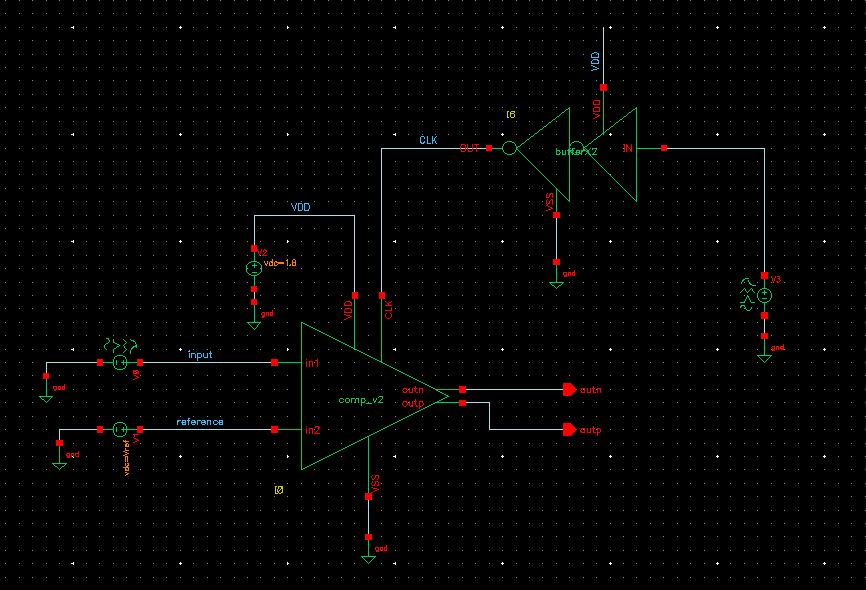
\includegraphics[width=0.8\textwidth]{img/tb1}
  \caption{Testbench of the SAR comparator}
  \label{fig:tb1}
 \end{figure}

 The purpose of the first testbench in \autoref{fig:tb1} is to verify the basic functionality of the comparator. That is, that $V\subb{out}^-=V\subb{DD}$ and $V\subb{out}^+=0$ when $V\subb{in}^->V\subb{in}^+$, and viceversa. The outputs are changed on the negative edge of the input clock and will retain their values during the entire negative half of the clock cycle. On the positive edge of the clock cycle, both outputs will be changed 0 and these values will be retained during the entire positive half of the clock cycle.

 \begin{figure}[!h]
  \centering
  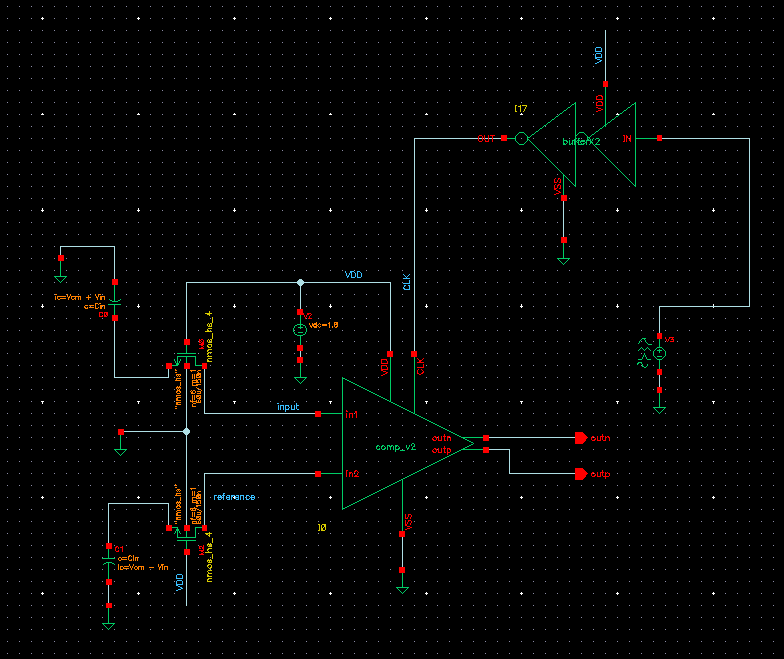
\includegraphics[width=0.8\textwidth]{img/tb2}
  \caption{Testbench of the SAR comparator}
  \label{fig:tb2}
 \end{figure}

The second testbench in \autoref{fig:tb2} is mainly useful for determining the amount of kickback noise. Kickback noise is a seen as a voltage drop or spike on the inputs as a result of capacitive coupling between the gate-drain and gate-source of transistors M1 and M2 in Fig. 1. This is an undesirable effect and can cause incorrect comparison results. For a comparator used in a SAR-ADC, the kickback noise must be less than $\frac{0.5/2^n}{2}$V, where $n$ is the desired amounts of bits of resolution that the ADC must be able to handle, in our case 5.\bigskip

In order to determine the common mode input voltage, we have to look at the sample-and-hold circuit which connects to in1 of the comparator.

 \begin{figure}[!h]
  \centering
  \tikzsetnextfilename{sh}
  \begin{tikzpicture}
 \draw (0,0) node[ground]{} to[european voltage source, v=$V\subb{in}$] ++ (0,2) --++(1,0) node[nmos, anchor=S, rotate=-90](q) {} (q.D)--++ (1,0) to[C, v^<=$V\subb{out}$] ++(0,-2) node[ground] {} (q.G) node[above] {$\varphi$};
\end{tikzpicture} 

  \caption{Simple sample \& hold circuit}
  \label{fig:sh}
 \end{figure}
 
 In \autoref{fig:sh} a simple sample-and-hold circuit is shown. In our case $V\subb{in}$ will be equal to $V\subb{cm}+V\subb{sample}$, that is, a common-mode voltage plus the voltage we are interested in sampling. in1 of the comparator is connected to the capacitor. The transistor used as a switch can be considered to be an n-channel MOSFET.

 The gate of the transistor will be driven by VDD=1.8, and in order for it conduct, the Vgs voltage must be equal to or greater than the threshold voltage. We can make the assumption that Vth=0.7 V. Further, we can make the assumption that the voltage drop between the drain and source is negligible.

 It’s easy to see that the voltage across the capacitor can’t be higher than 1.1 V, or else the transistor won’t conduct. Since Vsample will have a swing of \SI{0.5}{\volt_{pp}}, the maximum voltage present at the drain of the transistor will be $V\subb{cm} + 0.25$ V.

 Thus, to determine a suitable value for the common mode voltage, we use the following relation:
 \begin{equation}
  V\subb{cm} + 0.25=1.1
 \end{equation}

 Which gives a maximum common mode voltage of $V\subb{cm}=0.85$ V. In order to have a little more margin, we choose $V\subb{cm}=0.7$ V.

%Performing the simulation with testbench #2, using this common mode voltage and maximum value of \suVsample, we get:

 \subsection{Transient analysis}
 To verify the functionality of our circuit we perform a transient simulation where we expect to see the ouput of the comparator changing to high according to the relation $V\subb{in}^+\lessgtr V\subb{in}^-$.

 \begin{figure}[!h]
  \centering
  \caption{Transient analysis of the SAR comparator}
  \label{fig:transient}
  \tikzsetnextfilename{transient}
  \begin{tikzpicture}[trim axis left, trim axis right]
   \begin{axis}[
     x filter/.code={\pgfmathdivide{#1}{1e-9}},
     width=\textwidth, height=0.6\textwidth,
     enlarge x limits=0,
     xlabel=\si{\ns},
     ylabel=\si{\V},
     legend cell align={left},
     grid=both, minor grid style=dotted, minor y tick num = 5, minor x tick num=3,
    ]
    \addplot [thick, red] table[x=/input X, y=/input Y, col sep=comma] {./data/m1_transient.csv};
    \addlegendentry{Input};
    \addplot [thick, blue] table[x=/reference X, y=/reference Y, col sep=comma] {./data/m1_transient.csv};
    \addlegendentry{Reference};
    \addplot [thick, green] table[x=/outn X, y=/outn Y, col sep=comma] {./data/m1_transient.csv};
    \addlegendentry{Output};
   \end{axis}
  \end{tikzpicture}

 \end{figure}

 In \autoref{fig:transient} we can see the results of the transient simulation for two periods of a \SI{4}{\MHz} input sine wave. It is easy to check that the functionality of the comparator is as expected.
 \subsection{Kickback simulation}
 Untill this point, the effects of the capacitive coupling between the input and intermediate nodes of the comaprator has been ignored. In reality this effect can lead into significant errors due to the effect of the kickback.

 \begin{figure}[!h]
  \centering
  \caption{Close-up on the kickback noise effects}
  \label{fig:kickback_closeup}
  \tikzsetnextfilename{kickback_closeup}
  \begin{tikzpicture}[trim axis left, trim axis right, new spy style]
	   \begin{axis}[
	     x filter/.code={\pgfmathdivide{#1}{1e-9}},
	     width=\textwidth, height=0.6\textwidth,
	     enlarge x limits=0,
	     xlabel=\si{\ns},
	     ylabel=\si{\V},
	     legend cell align={left},
	     grid=both, minor grid style=dotted, minor y tick num = 4, minor x tick num=3,
	    ]
	    \addplot [thick, orange] table[x=/CLK X, y=/CLK Y, col sep=comma] {./data/m1_kickback.csv};
	    \addlegendentry{Clock};
	    \addplot [thick, red] table[x=/input X, y=/input Y, col sep=comma] {./data/m1_kickback.csv};
	    \addlegendentry{Input};
	    \addplot [thick, blue] table[x=/reference X, y=/reference Y, col sep=comma] {./data/m1_kickback.csv};
	    \addlegendentry{Reference};
	    \addplot [thick, green] table[x=/outn X, y=/outn Y, col sep=comma] {./data/m1_kickback.csv};
	    \addlegendentry{Output};
	    \coordinate (spypoint) at (axis cs:5,0.95);
	    \coordinate (spyloc) at (axis cs:7,0.3);
	   \end{axis}
	   \spy[size=2cm] on (spypoint) in node at (spyloc);
	  \end{tikzpicture}

 \end{figure}

 \autoref{fig:kickback_closeup} shows the effect of the so called kickback. As we can see the inputs, which are not supposed to change, present a significant variation due to the capacitive coupling through the parasitic capacitances of the transistors.
 To quantize this effec we use the following expression.

 \texttt{(ymax((vtime('tran "/input") - vtime('tran "/reference"))) - (2 * VAR("Vin")))}\bigskip

 \begin{figure}[!h]
  \centering
  \caption{Differential error generated by the kickback}
  \label{fig:kickback_diff}
  \tikzsetnextfilename{kickback_diff}
  \begin{tikzpicture}[trim axis left, trim axis right]
   \begin{axis}[
     x filter/.code={\pgfmathdivide{#1}{1e-9}},
     y filter/.code={\pgfmathdivide{#1}{1e-3}},
     width=\textwidth, height=0.6\textwidth,
     enlarge x limits=0,
     xlabel=\si{\ns},
     ylabel=$V\subb{in}^+-V\subb{in}^-\,/\,\si{\mV}$,
     legend cell align={left},
     grid=both, minor grid style=dotted, minor y tick num = 4, minor x tick num=3,
    ]
    \addplot [thick, red] table[x=diff X, y=diff Y, col sep=comma] {./data/m1_kickback.csv};
    \draw[thick, dashed] (axis cs:10,500.62) --++ (axis direction cs:2,0);
    \draw[thick, dashed] (axis cs:15,505.82) --++ (axis direction cs:-3,0);
    \draw[latex-latex] (12,500.62) -- (12,505.82) node[midway, right] {Kickback};
   \end{axis}
  \end{tikzpicture}

 \end{figure}

 This effect can be visualized in \autoref{fig:kickback_diff}.
 With the current sizes and biasing we obtain a kickback of only \SI{7.1}{\mV}.
 \subsection{Noise simulation}
 Untill this point, all the simulations were performed with noise-free components. The noise generated by the transistors and passive devices in the comparator can lead to significant error.

 To simulate this effects we enable the transient noise and we perform a transient analysis.

 \begin{figure}[!h]
  \centering
  \caption{Transient analysis with noise}
  \label{fig:noise}
  \tikzsetnextfilename{noise}
  \begin{tikzpicture}[trim axis left, trim axis right]
	   \begin{axis}[
	     x filter/.code={\pgfmathdivide{#1}{1e-9}},
	     width=\textwidth, height=0.6\textwidth,
	     enlarge x limits=0,
	     xlabel=\si{\ns},
	     ylabel=\si{\V},
	     legend cell align={left},
	     grid=both, minor grid style=dotted, minor y tick num = 5, minor x tick num=3,
	    ]
	    \addplot [thick, red] table[x=Vin X, y=Vin Y, col sep=comma] {./data/m1_noise-0.01.csv};
	    \addlegendentry{Input};
	    \addplot [thick, blue] table[x=REF X, y=REF Y, col sep=comma] {./data/m1_noise-0.01.csv};
	    \addlegendentry{Reference};
	    \addplot [thick, green] table[x=OUTN X, y=OUTN Y, col sep=comma] {./data/m1_noise-0.01.csv};
	    \addlegendentry{Output};
	   \end{axis}
	  \end{tikzpicture}

 \end{figure}
  
 When using a input signal of 0.5\% of the $V\subb{LSB}$ the results were identical to \autoref{fig:transient}, this means that the circuit works as expected. 
 
 In the other hand, when using a signal of 0.1\% of the $V\subb{LSB}$ the comparator was not working as expected, as can be seen in \autoref{fig:noise}. Note that the input signal cannot be seen in the plot since its amplitude was under 1 mV. This is a extermely low value so we dont have to worry about noise effects with this configuration.
 \subsection{Power Consumption}
 To obtain the power consumption of our circuit, we can measure the current that is being drawn from the $V\subb{DD}$ power supply. Since the behaviour of the comaprator is highly dynamic we cant use the DC values of those signals, integration over a period has to be done. Using this method we obtain a power consumption of \SI{76.82}{\uW}.
 \subsection{HDL Description}
 The Verilog-AMS description of the comparator can be seen in the Sample Code \ref{lst:comp}. To account for the propagation delay we used the functions \texttt{riseTime} and \texttt{fallTime} that are provided by Cadence ADE. We measured a rise time of \SI{574.4}{\ps} and a fall time of \SI{71.03}{\ps}. To simulate this propagation delay we added the delays expressions to the Verilog-AMS code (lines 21 and 29).
  \captionof{listing}{Verilog-AMS description of the comparator\label{lst:comp}}
  \inputminted{verilog}{../milestone1/comparator/comp_v2/verilogams/verilog.vams}
 
 \subsection{Layout}
 The layout was based on the layout that was provided. We just changed the sizes of the input transistors and adjusted the connections. Te final layout can be seen in \autoref{fig:layout}.

 \begin{figure}[h]
  \centering
  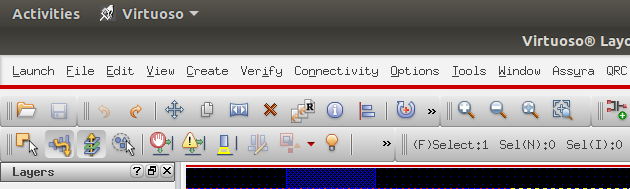
\includegraphics[angle=90, width=0.8\textwidth]{img/layout}
  \caption{Final layout of the ADC}
  \label{fig:layout}
 \end{figure}
 \section*{Milestone 2}
 \setcounter{section}{2}
 \setcounter{subsection}{0}
 In this milestone we will choose the reference voltage that the SAR ADC is going to use as well as calculating the resolution of it.
 \subsection{Resolution of the SAR ADC}
 From the simulation results we got a kickback noise of 7.1 mV, and we know that the kickback noise must be at least half of the LSB. We can write this condition as
 \begin{equation}
  V\subb{glitch} < \frac{V\subb{full swing}\cdot 0.5}{2^N}
 \end{equation}
 If we solve this for N, we get
 \begin{equation}
  N=\log_2\!\left(\frac{V\subb{full swing}\cdot 0.5}{0.0071}\right)=5.138
 \end{equation}
 Which rounded down is 5, which is the maximum resolution that this ADC can support with this comparator.
 \subsection{Voltage reference selection}
 For the voltage reference, we choose $V\subb{ref}=500$ mV. This is the maximum anticipated value on the input. According to the behavioral modeling tutorial, the common mode needs to be half of this. This means we might have to revise our initial choice of $V\subb{cm}=700$ mV as we go along in this process
 \section*{Milestone 3}
 \setcounter{section}{3}
 \setcounter{subsection}{0}
 For this milestone we need to analyze the behaviour of the sucecssive approximation register and determine the sample rate of the ADC.
 \subsection{Resolution of the SAR ADC}
 In order to obtain a resolution of 5 bits, we need to modify the provided Verilog code to adapt it to 5 bits resolution. This modification is achieved by adding a 5th state to the state machine performing the binary search algorithm. This modification can be seen in Sample Code \ref{lst:sar}.
 
  \captionof{listing}{Verilog description of the SAR\label{lst:sar}}
  \inputminted{verilog}{../IL2239_SAR_ADC/SAR4/functional/verilog.v}
 
 \subsection{Top level simulations}
 After doing the modifications to the SAR description, we can proceed to perform a top level simulation of all the blocks in our system. To do that we use the testbench seen in \autoref{fig:sar_tb}.  The DAC used in the feedback loop of the SAR ADC (see \autoref{fig:sar}) provided consisted only of 4 bits so an aditional branch of capacitors. The final schematic of the DAC can be seen in \autoref{fig:dac}.\bigskip

 Performing a transient simulation with an input signal and observing the output of the ADC we can see the conversion results and observe the offset between the reconstructed signal and the input signal. This results can be seen in \autoref{fig:sinusoidal-conversion}. To reconstruct the digital signal an ideal DAC was used.

 \begin{figure}[h]
  \centering
  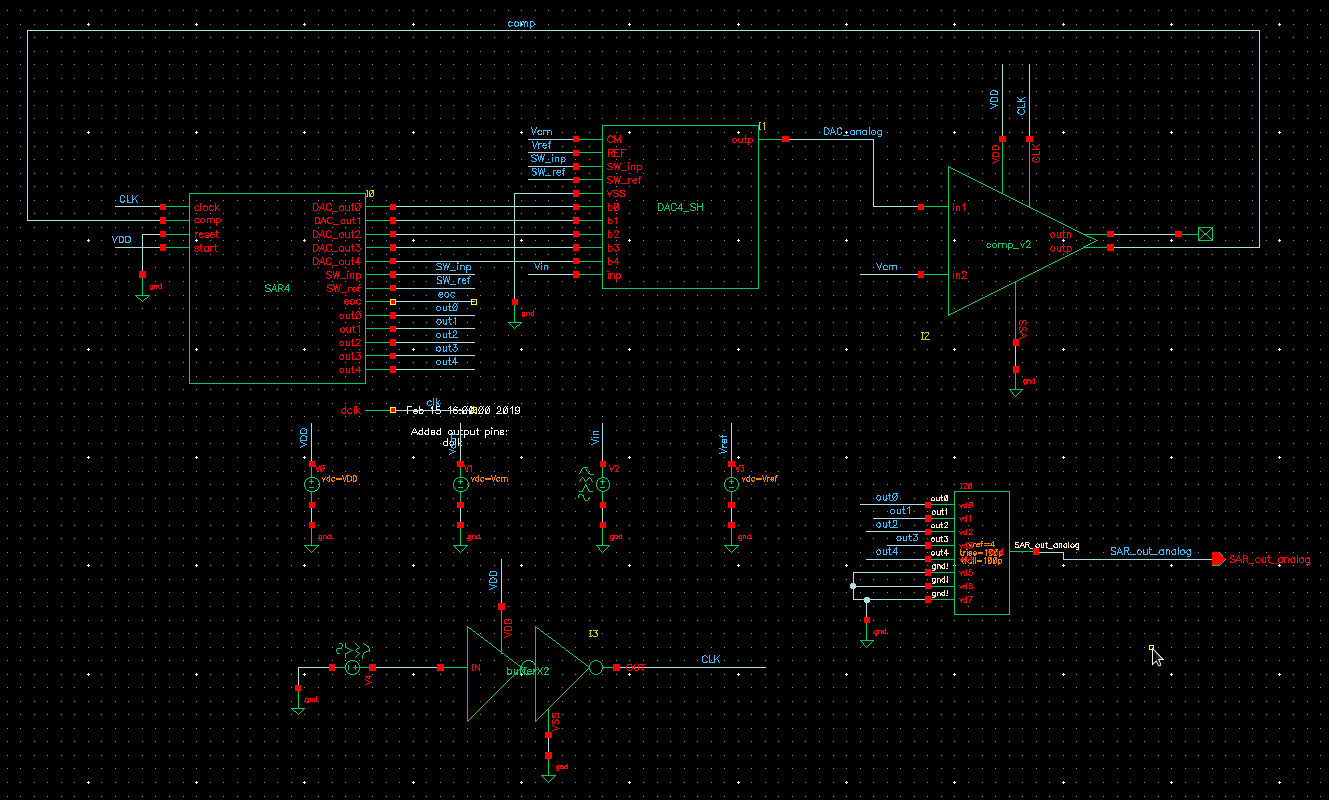
\includegraphics[width=0.8\textwidth]{./img/m3_schematic}
  \caption{SAR testbench}
  \label{fig:sar_tb}
 \end{figure}

 \begin{figure}[h]
  \centering
  \tikzsetnextfilename{sinusoidal-conversion}
  \begin{tikzpicture}[timing/unit=1cm]
 \begin{axis}[
   name=analog,
   x filter/.code={\pgfmathdivide{#1}{1e-9}},
   width=\textwidth, height=0.4\textwidth,
   enlarge x limits=0,
   xlabel=\si{\ns},
   ylabel=\si{\V},
   legend cell align={left},
   grid=both, minor grid style=dotted, minor y tick num = 5, minor x tick num=3,
  ]
  \addplot [thick, red] table[x=VinX, y=VinY, col sep=comma] {./data/m3_matlab_decimated.csv};
  \addlegendentry{Input signal};
  \addplot [thick, blue] table[x=SAR_out_analogX, y=SAR_out_analogY, col sep=comma] {./data/m3_matlab_decimated.csv};
  \addlegendentry{Output signal};
 \end{axis}
 \begin{axis}[
   name=clk,
   anchor=north,
   at={($(analog.south)-(0,8ex)$)},
   width=\textwidth, height=0.15\textwidth,
   x filter/.code={\pgfmathdivide{#1}{1e-9}},
   enlarge x limits=0,
   axis line style={draw=none},
   tick style={draw=none}, ytick=\empty, xtick=\empty,
   ylabel=CLK, ylabel style={rotate=-90},
  ]
  \addplot [thick] table[x=clkX, y=clkY, col sep=comma] {./data/m3_matlab_clk.csv};
 \end{axis}
 \begin{axis}[
   name=out0,
   anchor=north,
   at={($(clk.south)-(0,2ex)$)},
   width=\textwidth, height=0.15\textwidth,
   x filter/.code={\pgfmathdivide{#1}{1e-9}},
   enlarge x limits=0,
   axis line style={draw=none},
   tick style={draw=none}, ytick=\empty, xtick=\empty,
   ylabel={out[0]}, ylabel style={rotate=-90},
  ]
  \addplot [thick] table[x=out0X, y=out0Y, col sep=comma] {./data/m3_matlab_decimated.csv};
 \end{axis}
 \begin{axis}[
   name=out1,
   anchor=north,
   at={($(out0.south)-(0,2ex)$)},
   width=\textwidth, height=0.15\textwidth,
   x filter/.code={\pgfmathdivide{#1}{1e-9}},
   enlarge x limits=0,
   axis line style={draw=none},
   tick style={draw=none}, ytick=\empty, xtick=\empty,
   ylabel={out[1]}, ylabel style={rotate=-90},
  ]
  \addplot [thick] table[x=out1X, y=out1Y, col sep=comma] {./data/m3_matlab_decimated.csv};
 \end{axis}
 \begin{axis}[
   name=out2,
   anchor=north,
   at={($(out1.south)-(0,2ex)$)},
   width=\textwidth, height=0.15\textwidth,
   x filter/.code={\pgfmathdivide{#1}{1e-9}},
   enlarge x limits=0,
   axis line style={draw=none},
   tick style={draw=none}, ytick=\empty, xtick=\empty,
   ylabel={out[2]}, ylabel style={rotate=-90},
  ]
  \addplot [thick] table[x=out2X, y=out2Y, col sep=comma] {./data/m3_matlab_decimated.csv};
 \end{axis}
 \begin{axis}[
   name=out3,
   anchor=north,
   at={($(out2.south)-(0,2ex)$)},
   width=\textwidth, height=0.15\textwidth,
   x filter/.code={\pgfmathdivide{#1}{1e-9}},
   enlarge x limits=0,
   axis line style={draw=none},
   tick style={draw=none}, ytick=\empty, xtick=\empty,
   ylabel={out[3]}, ylabel style={rotate=-90},
  ]
  \addplot [thick] table[x=out3X, y=out3Y, col sep=comma] {./data/m3_matlab_decimated.csv};
 \end{axis}
 \begin{axis}[
   name=out4,
   anchor=north,
   at={($(out3.south)-(0,2ex)$)},
   width=\textwidth, height=0.15\textwidth,
   x filter/.code={\pgfmathdivide{#1}{1e-9}},
   enlarge x limits=0,
   axis line style={draw=none},
   tick style={draw=none}, ytick=\empty, xtick=\empty,
   ylabel={out[4]}, ylabel style={rotate=-90},
  ]
  \addplot [thick] table[x=out4X, y=out4Y, col sep=comma] {./data/m3_matlab_decimated.csv};
 \end{axis}
 \draw (out4.south west) ++ (0,-10ex) coordinate (en);
 \timing at (en) {D{00}D{14}D{25}D{29}D{22}D{10}2D{00}D{03}D{15}D{26}D{28}D{22}D{10}0.5D{0}};
 \draw (en) ++ (0,3ex)node[left] {out[4:0]};
\end{tikzpicture}

  \caption{Waveforms from a sinusoidal signal conversion}
  \label{fig:sinusoidal-conversion}
 \end{figure}

 \begin{figure}[h]
  \centering
  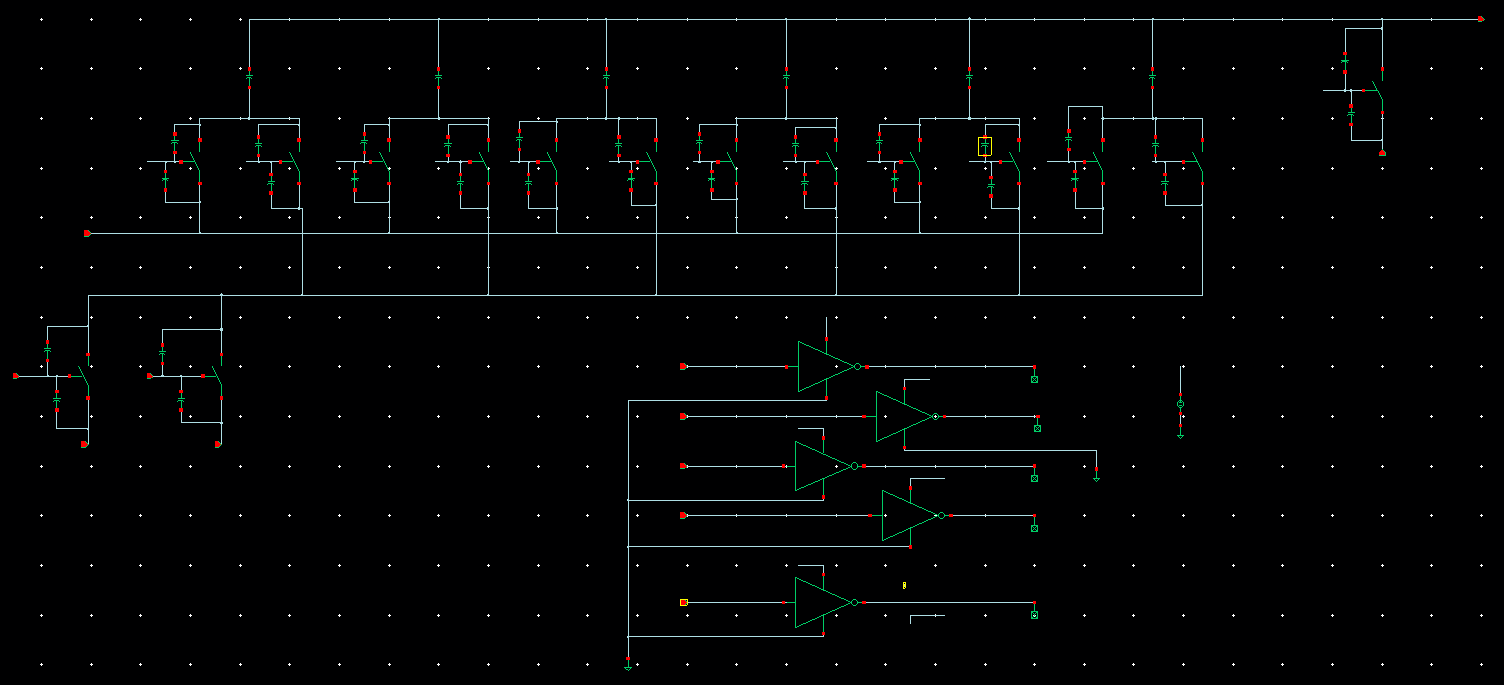
\includegraphics[width=0.8\textwidth]{./img/m3_sar}
  \caption{DAC Schematic}
  \label{fig:dac}
 \end{figure}

 \begin{figure}[h]
  \centering
  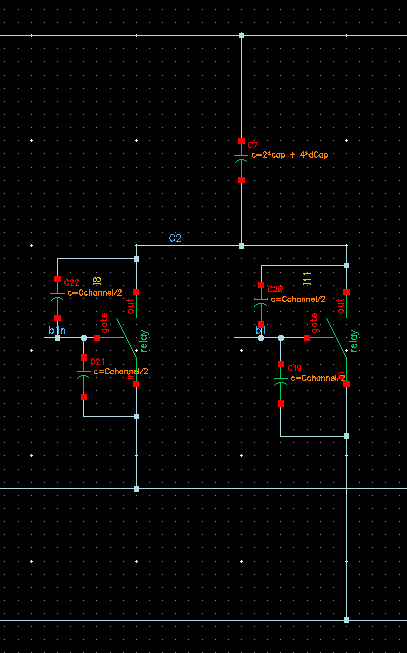
\includegraphics[width=0.8\textwidth]{./img/m3_sar_closeup}
  \caption{SAR testbench}
  \label{fig:dac_cp}
 \end{figure}
 \subsection{Sampling Rate}
 To determine the sampling rate of the ADC we need to analyze the how the convertion is done. The SAR takes $N$ clock samples to converge to a final value and an aditional two clocks are needed for the setteling of the signal and additional logic and reset phases. Thus we can expres the sampling rate of our ADC as.
 \begin{equation}
  f\subb{sample} = \frac{f\subb{clk}}{N+2}
 \end{equation}
 In our project $f\subb{clk}=\SI{100}{\MHz}$ and $N=5$ so $f\subb{sample}=\SI{14.29}{\MHz}$.
 %\section*{Milestone 4}
 %\setcounter{section}{4}
 %\setcounter{subsection}{0}
\end{document}
